\appendix

\chapter{Anexo: Listado de piezas}\label{anexopiezas}

\begin{table}[h]
\centering
\begin{tabular}{ >{\centering\arraybackslash}m{4cm} >{\arraybackslash}m{2cm}  >{\centering\arraybackslash}m{1cm}  >{\centering\arraybackslash}m{4cm}}
\hline
Imagen & Archivo & Cantidad & Observaciones  \\
\hline \hline
\medskip 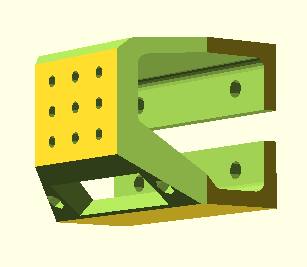
\includegraphics[width=30mm]{figuras/antebrazo} & antebrazo.stl & x2 & Se imprimen dos iguales, son sim�tricas \\ \hline 
\medskip 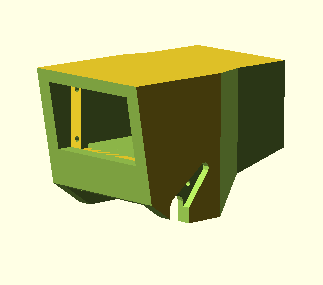
\includegraphics[width=30mm]{figuras/cabeza} & cabeza.stl & x1 &  \\ \hline
\medskip 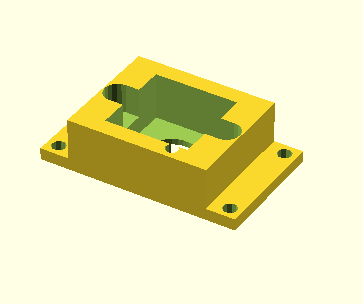
\includegraphics[width=30mm]{figuras/chasislifecam} & chasislifecam.stl & x1 &  \\ \hline
\medskip 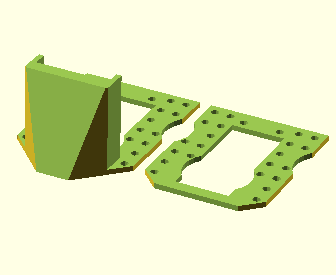
\includegraphics[width=30mm]{figuras/cintura} & cintura.stl & x1 & El archivo incluye las dos partes de la pieza  \\ \hline
\hline
\end{tabular}
\caption{Lista de piezas 1/4}
\label{tabl}
\end{table}

\begin{table}[h]
\centering
\begin{tabular}{ >{\centering\arraybackslash}m{4cm} >{\arraybackslash}m{2cm}  >{\centering\arraybackslash}m{1cm}  >{\centering\arraybackslash}m{4cm}}
\hline
Imagen & Archivo & Cantidad & Observaciones  \\
\hline \hline
\medskip 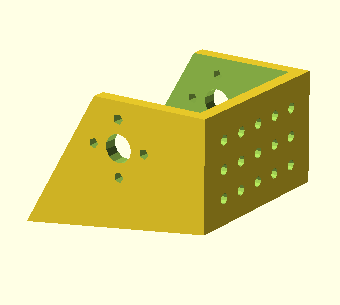
\includegraphics[width=30mm]{figuras/codo} & codo.stl & x2 & Incluye versi�n A (izquierda) y B (derecha) \\ \hline
\medskip 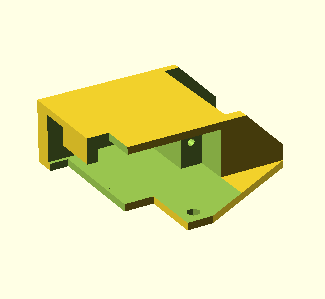
\includegraphics[width=30mm]{figuras/cuello} & cuello.stl & x1 &  \\ \hline 
\medskip 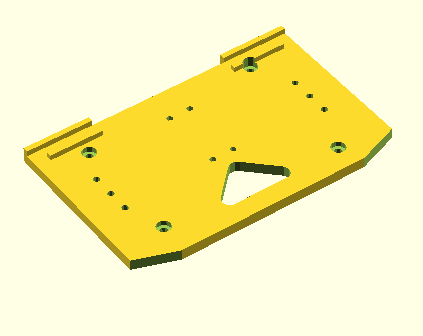
\includegraphics[width=30mm]{figuras/espalda} & espalda.stl & x1 &  \\ \hline
\medskip 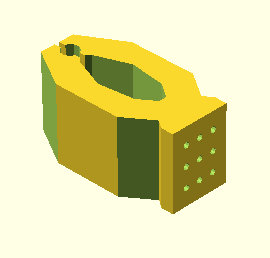
\includegraphics[width=30mm]{figuras/gripper} & gripper.stl & x2 & Se imprimen dos iguales, son sim�tricas \\ \hline
\medskip 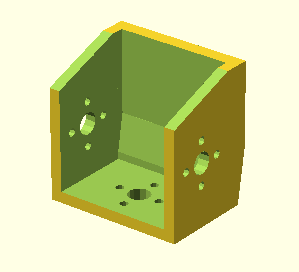
\includegraphics[width=30mm]{figuras/hombro} & hombro.stl & x1 & Se imprimen dos iguales, son sim�tricas \\ \hline
\hline
\end{tabular}
\caption{Lista de piezas 2/4}
\label{tabl}
\end{table}

\begin{table}[h]
\centering
\begin{tabular}{ >{\centering\arraybackslash}m{4cm} >{\arraybackslash}m{2cm}  >{\centering\arraybackslash}m{1cm}  >{\centering\arraybackslash}m{4cm}}
\hline
Imagen & Archivo & Cantidad & Observaciones  \\
\hline \hline
\medskip 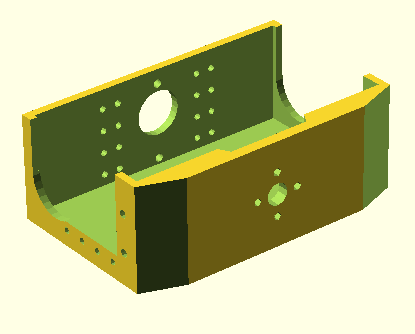
\includegraphics[width=30mm]{figuras/pecho} & pecho.stl & x1 &  \\ \hline
\medskip 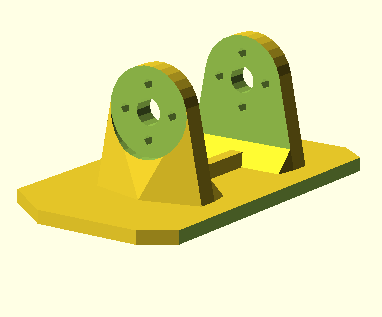
\includegraphics[width=30mm]{figuras/pie} & pie.stl & x2 & Incluye versi�n A (izquierda) y B (derecha) \\  \hline
\medskip 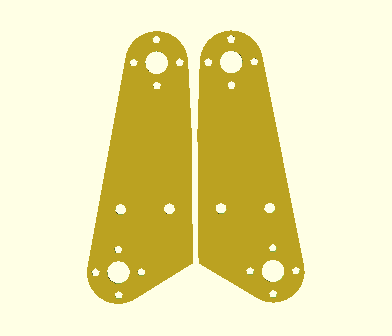
\includegraphics[width=30mm]{figuras/pierna1} & pierna1.stl & x2 &  Se imprimen dos iguales, son sim�tricas. El archivo incluye dos piezas \\ \hline
\medskip 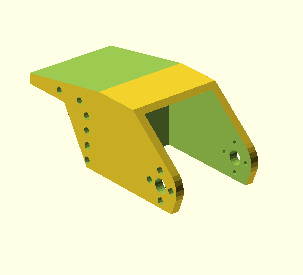
\includegraphics[width=30mm]{figuras/pierna2} & pierna2.stl & x2 &  Se imprimen dos iguales, son sim�tricas \\ \hline
\medskip 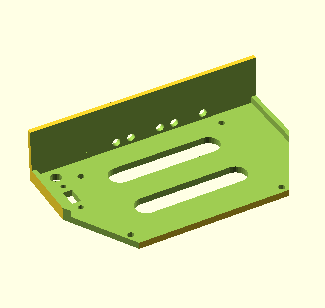
\includegraphics[width=30mm]{figuras/protector} & protector.stl & x1 &  \\ \hline
\hline
\end{tabular}
\caption{Lista de piezas 3/4}
\label{tabl}
\end{table}

\begin{table}[h]
\centering
\begin{tabular}{ >{\centering\arraybackslash}m{4cm} >{\arraybackslash}m{2cm}  >{\centering\arraybackslash}m{1cm}  >{\centering\arraybackslash}m{4cm}}
\hline
Imagen & Archivo & Cantidad & Observaciones  \\
\hline \hline
\medskip 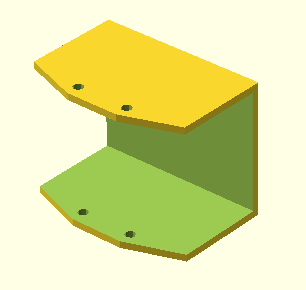
\includegraphics[width=30mm]{figuras/soportebat} & soporteBateria.stl & x1 &  \\ \hline
\medskip 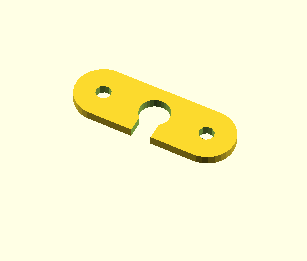
\includegraphics[width=30mm]{figuras/tapacabeza} & tapaCabeza.stl & x1 &  \\ \hline
\medskip 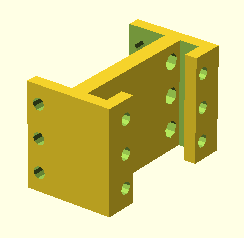
\includegraphics[width=30mm]{figuras/tobillo} & tobillo.stl & x2 &  Se imprimen dos iguales, son sim�tricas \\ \hline
\hline
\end{tabular}
\caption{Lista de piezas 4/4}
\label{tabl}
\end{table}


